
\chapter{関連する技術や先行研究}
\label{related}

%関連研究では,
%* 車両のセンサーを用いる駐車場内の最適化手法
%* 車載アプリケーションプラットフォーム
%(DICOMO論文からそのままパクってくる)
%について述べる$\cdot$

ICT環境の発達によって従来の敷設センサーに頼らない駐車場の効率化が多く研究されている.
本章では駐車場の効率化手法を分類し,本提案手法が担う役割に関して記述する.

\section{駐車場空き状況センシング手法}
\label{legacy-sensing}
本節では様々な駐車場の空き状況センシング手法について記述する.
\subsection{敷設センサーによるセンシング}
日本において従来より広く導入されている手法である.運営主体によって路側に常設された機器がセンシングを行う.そのため,管理$\cdot$利活用$\cdot$情報の開示にかかるコストを運営者が負担する場合が多い.
これらのセンサーによって得られた満空情報についてどこまでの情報を開示し提供するかは運用主体の裁量で決まる.以下に主な敷設センサーを列挙する.


\begin{itemize}
					
	\item フラップ式センサー\\
	      \begin{figure}
	      	\centering
	      	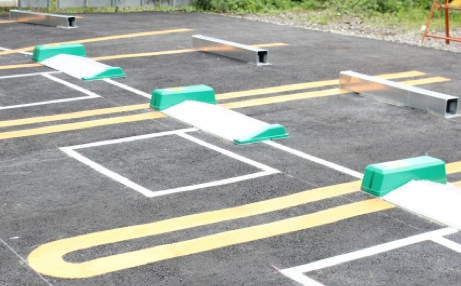
\includegraphics[width=7cm]{fig/flap.png}
	      	\caption{フラップ式センサーの設置された駐車区画\protect \footnotemark}
	      	\label{flap}
	      \end{figure}
	      \footnotetext{\url{https://www.photo-ac.com/main/detail/505568}より引用 最終確認日 2018年1月17日}
	      都市部の地上型駐車場で一般に普及しているセンシング手法である(図\ref{flap}).利用車両の未払いを防ぐ働きも担っている.
	      	      	      	      	      
	\item モニタリングセンサーノード\\
	      \begin{figure}
	      	\centering
	      	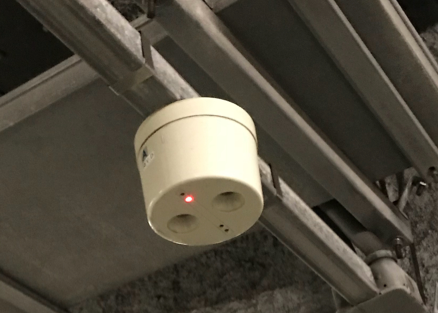
\includegraphics[width=7cm]{fig/sensor-node.png}
	      	\caption{羽田空港国際線ターミナル駐車場に設定されているモニタリングセンサーノード \protect \footnotemark}
	      	\label{sensor-node}
		  \end{figure}
		  \footnotetext{羽田空港国際線ターミナル駐車場にて2017年11月撮影}
	      大型の階層型駐車場で用いられている手法である(図\ref{sensor-node}).それぞれの駐車枠上部に常設機器を設置し空き状況をセンシングする.利用者は施設内に設置されたモニターで各駐車区画の空き状況を確認出来るケースが多い.
	      	      	      	      	      
	\item 監視カメラを用いた画像認識\\
	      \begin{figure}
	      	\centering
	      	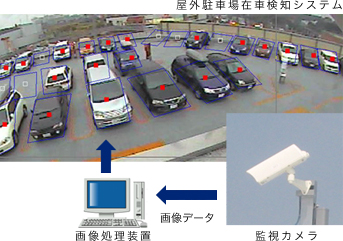
\includegraphics[width=7cm]{fig/camera.png}
	      	\caption{監視カメラによる満空情報の認識システム\protect \footnotemark}
	      	\label{camera}
	      \end{figure}
	      \footnotetext{株式会社ニチゾウテック 駐車場誘導管制設  \url{http://www.nichizotech.co.jp/products/04parking/index.html}より引用 最終確認日2017年1月17日}
	      監視カメラの映像から各区画の満空情報を認識する手法である(図\ref{camera}).近年急速に導入されている.ステレオカメラを用いる手法も研究されており,山崎ら\cite{Yamazaki}によれば従来型のシステムよりも高い精度で車両を認識することが可能になるとされている.
\end{itemize}

運営主体によっては上記のセンサーで得られた満空情報を独自のプラットフォームでユーザーに公開する場合がある.例えばタイムズ24株式会社では,自社が運営している駐車場の大まなか満空情報をWEBサービスを用いてユーザーに公開している\cite{times}.図\ref{times-fig}にタイムズ24株式会社による検索サービスのスクリーンショットを示す.一方でユーザーが同じ地域の空き駐車場を検索するためには,運営主体ごとにそれぞれ独立したWEBサイトにアクセスする必要があり利便性を欠く.また設置$\cdot$運営に関わるコストを全て運営主体が担わなくてはならないため,運営コストを割くことが出来ない学校のような非営利団体が運営する駐車場での導入は困難である.


\begin{figure}
	\centering
	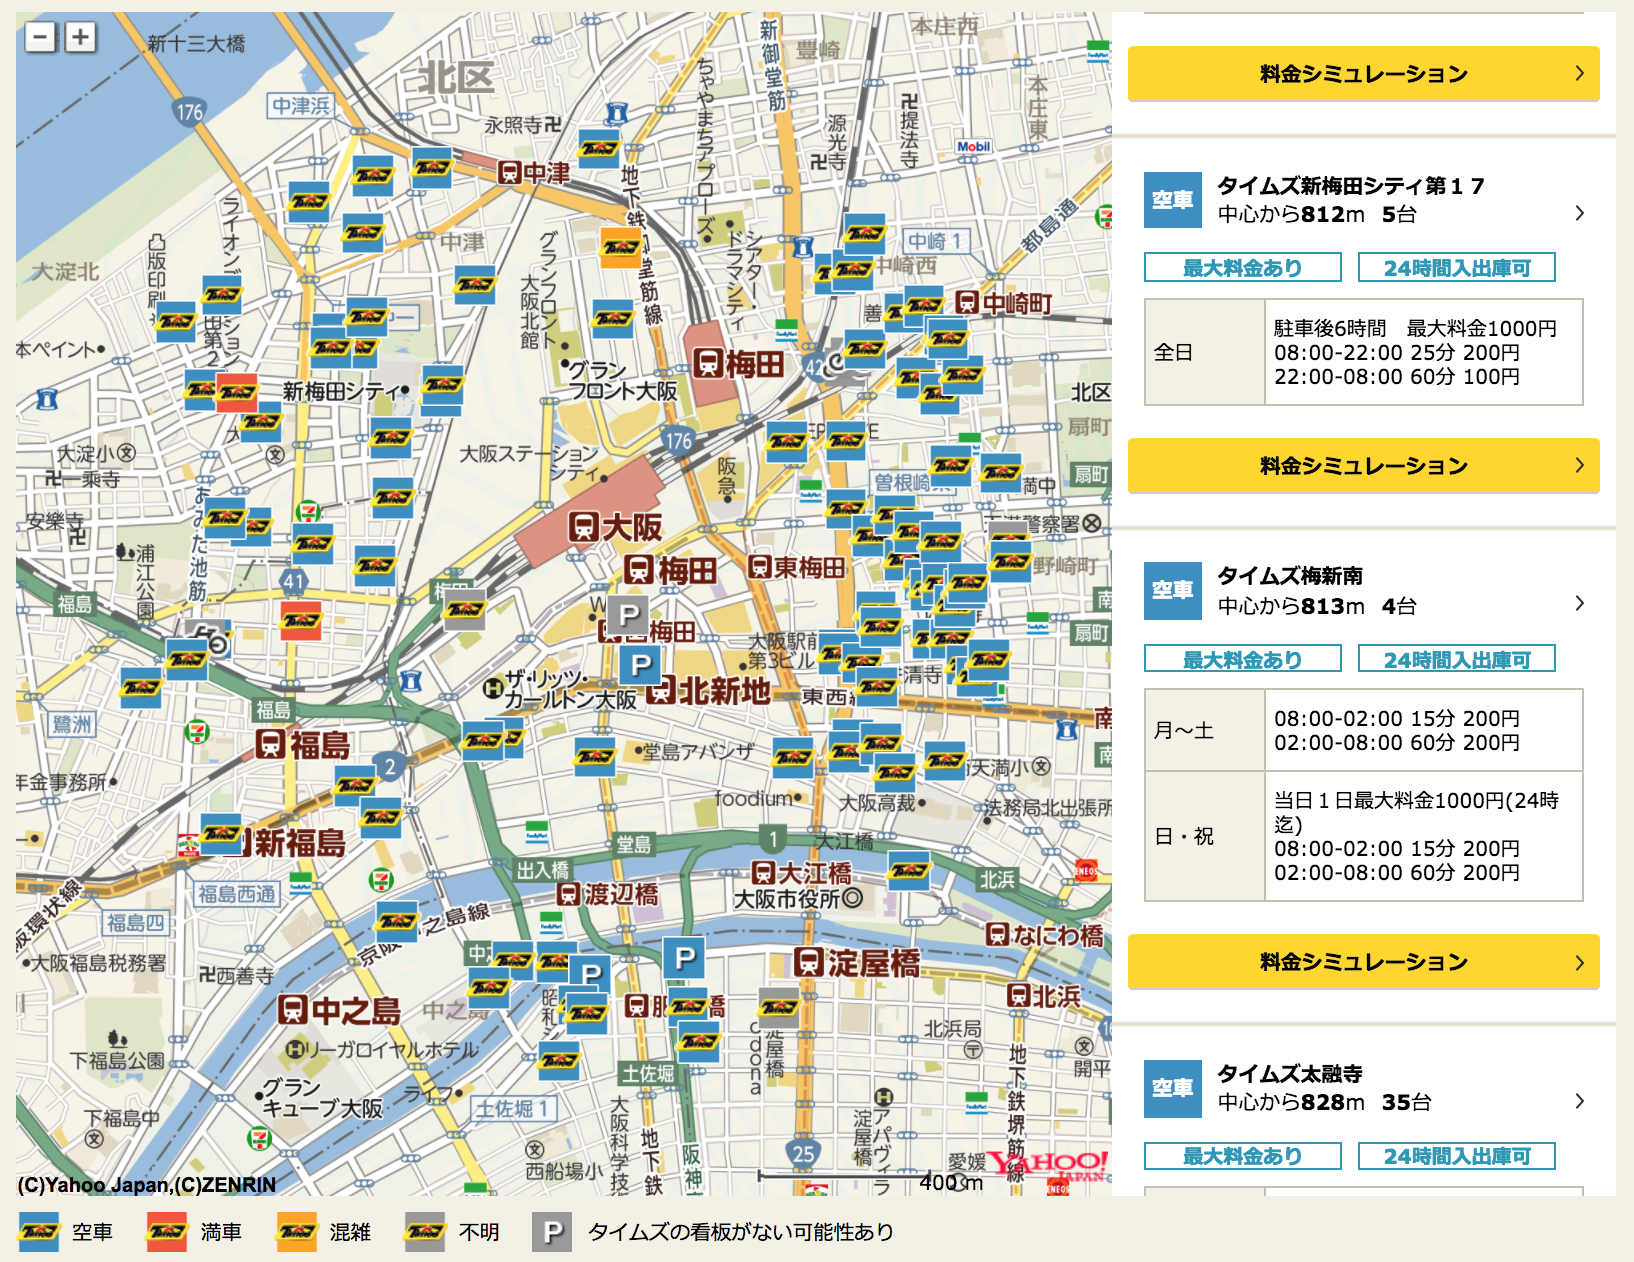
\includegraphics[width=12cm]{fig/times-fig.png}
	\caption{タイムズ24株式会社 タイムズ駐車場検索 \protect \footnotemark}
	\label{times-fig}
\end{figure}
\footnotetext{\url{https://times-info.net/}より引用 最終確認日2017年1月17日}

\section{車両のセンサーを用いる駐車場内の最適化手法}
従来,駐車場内の満空管理や車両の誘導は路側に設置されたセンサーやインジケータを用いる手法が一般的であった.
しかしながら近年ではVANETや衛星測位システム,携帯電話回線網を用いる手法が提案されている.


\subsection{VANET技術}
本節ではEliasらによるサーベイ\cite{Elias}を引用し,多くの駐車場内の効率化システムを実現する技術であるVANETについての概略について述べる.




\subsubsection{概要}
車々間$\cdot$路車間で構成されるアドホックネットワークを,一般してVANET(Vehicle Adhock Network)と呼称する.
VANETに参加する車両には車載通信装置(OBU)が装備され,他のOBUや路側装置(RSU)との無線通信が可能である.
図\ref{vanet}にVANETでの通信の概要を示す.


車両のOBU同士の通信はV2V(Vehicle to Vehicle)通信と呼ばれ,タイムクリティカルな危険予知情報の伝達に用いられる.

一方で,路側に設置されたRSUとOBUとの通信はV2I(Vehicle to infrastructure)通信と呼ばれる.これは主にRTK-GPS\cite{RTK}のような数センチ単位の正確な位置情報を車両側に提供するプロトコルや,交通信号機や指示板の情報の伝達に用いられる.

また,OBU$\cdot$RSUを伝播して情報を伝える通信をルーティングベース(RB)通信と呼ぶ.RB通信を用いて駐車場内の満空状況を車両のみで伝達する手法が山下らによって提案されている\cite{Yamashita}.




\begin{figure}
	\centering
	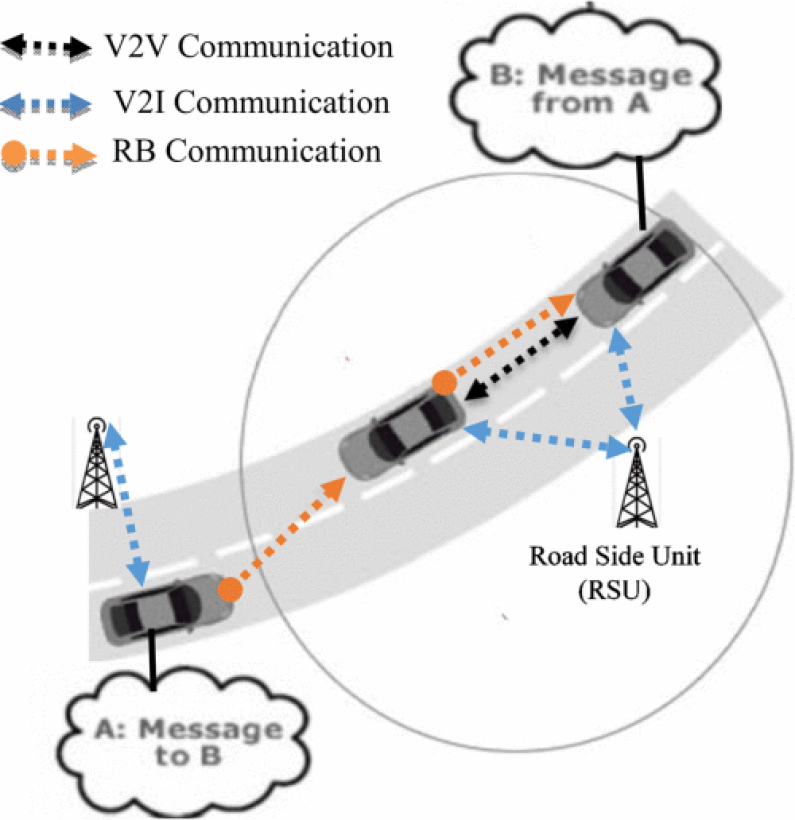
\includegraphics[width=10cm]{fig/vanet.png}
	\caption{VANETのネットワーク図 \protect \footnotemark}
	\label{vanet}
\end{figure}
\footnotetext{Eliasらの資料\cite{Elias}より引用}


\subsubsection{想定する無線通信規格}
VANETは各国の法規制や電波環境に併せて様々な無線通信規格での運用が議論されている.

\begin{itemize}
	\item IEEE 802.11p\cite{802.11p-official}\\
	      \label{802.11p}
	      IEEEによって定められたITS用の国際的な無線通信規格である.基本的には5.9GHz帯を用いる.
	      米国を中心に標準化$\cdot$普及が行われているが,日本においてはノンストップ自動料金支払いシステム(ETC)に代表される狭域通信(DSRC)\cite{DSRC}専用として利用されるARIB STD-T75\cite{ARIB}と,周波数帯が近いため導入が遅れている\cite{802.11p-sup}.
	\item 携帯電話回線\\
	      ITUによって標準化されている2G,2.5G,3G,4Gなどの携帯電話回線網\cite{itu}は信頼性の高いセキュリティと広いカバレッジを得られるメリットがある反面,リアルタイム性に優れないというデメリットがある.一方で,近年では次世代規格である低遅延$\cdot$多数同時接続を目標とした5Gの策定も進んでおり,VANETを用いた安全運転支援や自動運転車両の遠隔制御などでの活用が期待されている\cite{5G-soumu}.
	\item Unified wireless access\\
	      ISO/TC/204/WG16\cite{iso-tc-204}にて既存の無線通信を統合的に扱うための標準仕様として策定されたのがCALM M5\cite{CALM}である.これはIEEE802.11pをベースに携帯電話回線の技術を加えて構成されており,スループットの増加や冗長化が可能になっている.
\end{itemize}



\subsection{VANETを用いた駐車場の効率化手法}
\label{sensing-by-vanet}
VANETには安全運転支援システムやプラトゥーニングなどへの応用例が目立つが,駐車場の効率化手法としても取り入れられつつある.本節ではVANETを基盤技術として用いる関連研究に関して述べる.

\subsubsection{SPARK}

R.Luらによって提案されたSPARK\cite{Spark}は,VANETを介して全ての利用車両に対して駐車場所を指定していくプラットフォームである.図\ref{spark}は本手法が用いるV2I通信を簡潔に表したものである.中央システムが利用車両に電子チケットを発行して駐車区画の占有権を与える役割の他に,その区画へのナビゲーション機能や車両盗難防止機能なども提案している.SPARKでは,電子チケットを発行した車両がそこに駐車したと仮定することで,中央システムが駐車場全体の満空情報の監視$\cdot$提供することを想定している.しかしながら,路側センサーの設置と中央システムの運営を運営主体が行う必要性があるという従来型満空センシングアーキテクチャが抱える問題をそのまま継承している.

\begin{figure}
	\centering
	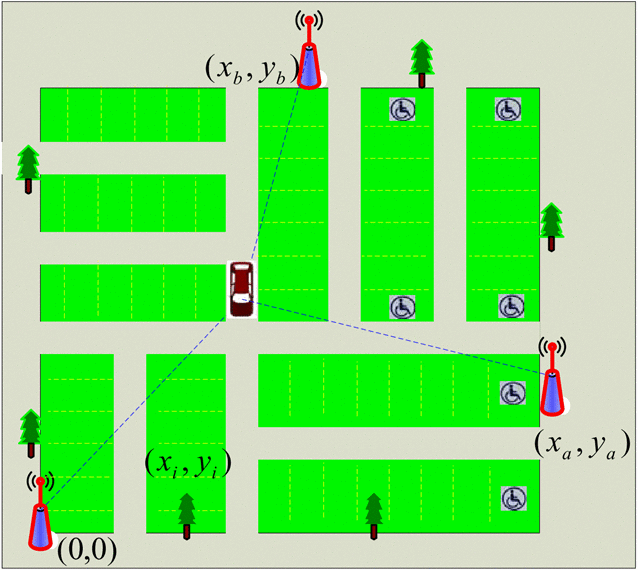
\includegraphics[width=10cm]{fig/spark-1.png}
	\caption[R.Luらにより提案されたSPARK手法の概念図]{SPARK手法ではRSUを用いたV2I通信を活用することで,利用車両への駐車枠の誘導や情報提供を可能にしている \protect \footnotemark}
	\label{spark}
\end{figure}
\footnotetext{SPARKの資料\cite{Spark}より引用}


\subsubsection{V2V通信のみで情報を伝達する手法}

山下らは,車両の近接センサーによって得られた近傍駐車枠の満空情報をVANETを用いて伝達し,ネットワークに参加している車両内で駐車場全体の満空情報を共有する手法を提案している\cite{Yamashita}.各車両が路面に書かれた駐車区画番号を車載カメラによる画像認識することで位置情報を特定することを想定している.中央のシステムに頼ること無く駐車場内の効率化が図れる一方,駐車場内のネットワークモデルを前提知識として共有しているため,運営者による詳細なネットワークモデルの提供が不可欠であると言える.

\subsubsection{VANETによる位置測位と路側から情報共有によるナビゲーションシステム}

孫らは,路車間通信によって車両の位置情報から割り出された最適な駐車区画への経路を利用者にナビゲーションする手法を提案している\cite{Sun-Kenmochi}.中央のシステムがRSUを介して車両の位置情報を収集し,満空情報と駐車成功度を車両に広報する.これらの情報を基に,新しく駐車場内に進入した車両に対して,最適な駐車区画の割当$\cdot$ナビゲーションが行われる.システムを搭載した車両が少ない場合でも駐車までの時間が短縮される点が特徴である.一方,このアーキテクチャでも,事前に中央システム$\cdot$利用車両が駐車場内のネットワークモデルを把握している必要がある.



\subsection{位置情報システムと携帯電話線網を用いたセンシング手法}

近年,位置情報システムを用いたサービスやアプリケーションがより身近なものになっている.
位置情報システムで最も広く利用されているのがGPSに代表される全球測位衛星システム(GNSS)である.GPSの測位位置の誤差は通常4.9Mほどであり\cite{gps-gov},近年では準天頂衛星システム(QZSS)による補正を受けることで理論上1M以内の高精度を見込める\cite{michibiki}.また,広帯域な携帯電話回線を安価に導入できる環境が整ったことで,携帯電話回線を備えた車載機器を用いて位置情報の収集を行う手法も一般的になっている.


本項では位置情報システムと携帯電話回線網によって満空情報を推定する手法について述べる.

\subsubsection{車載センサーと携帯電話回線網を用いた路上駐車枠の空き情報検知手法}

\begin{figure}[htb]
	\centering
	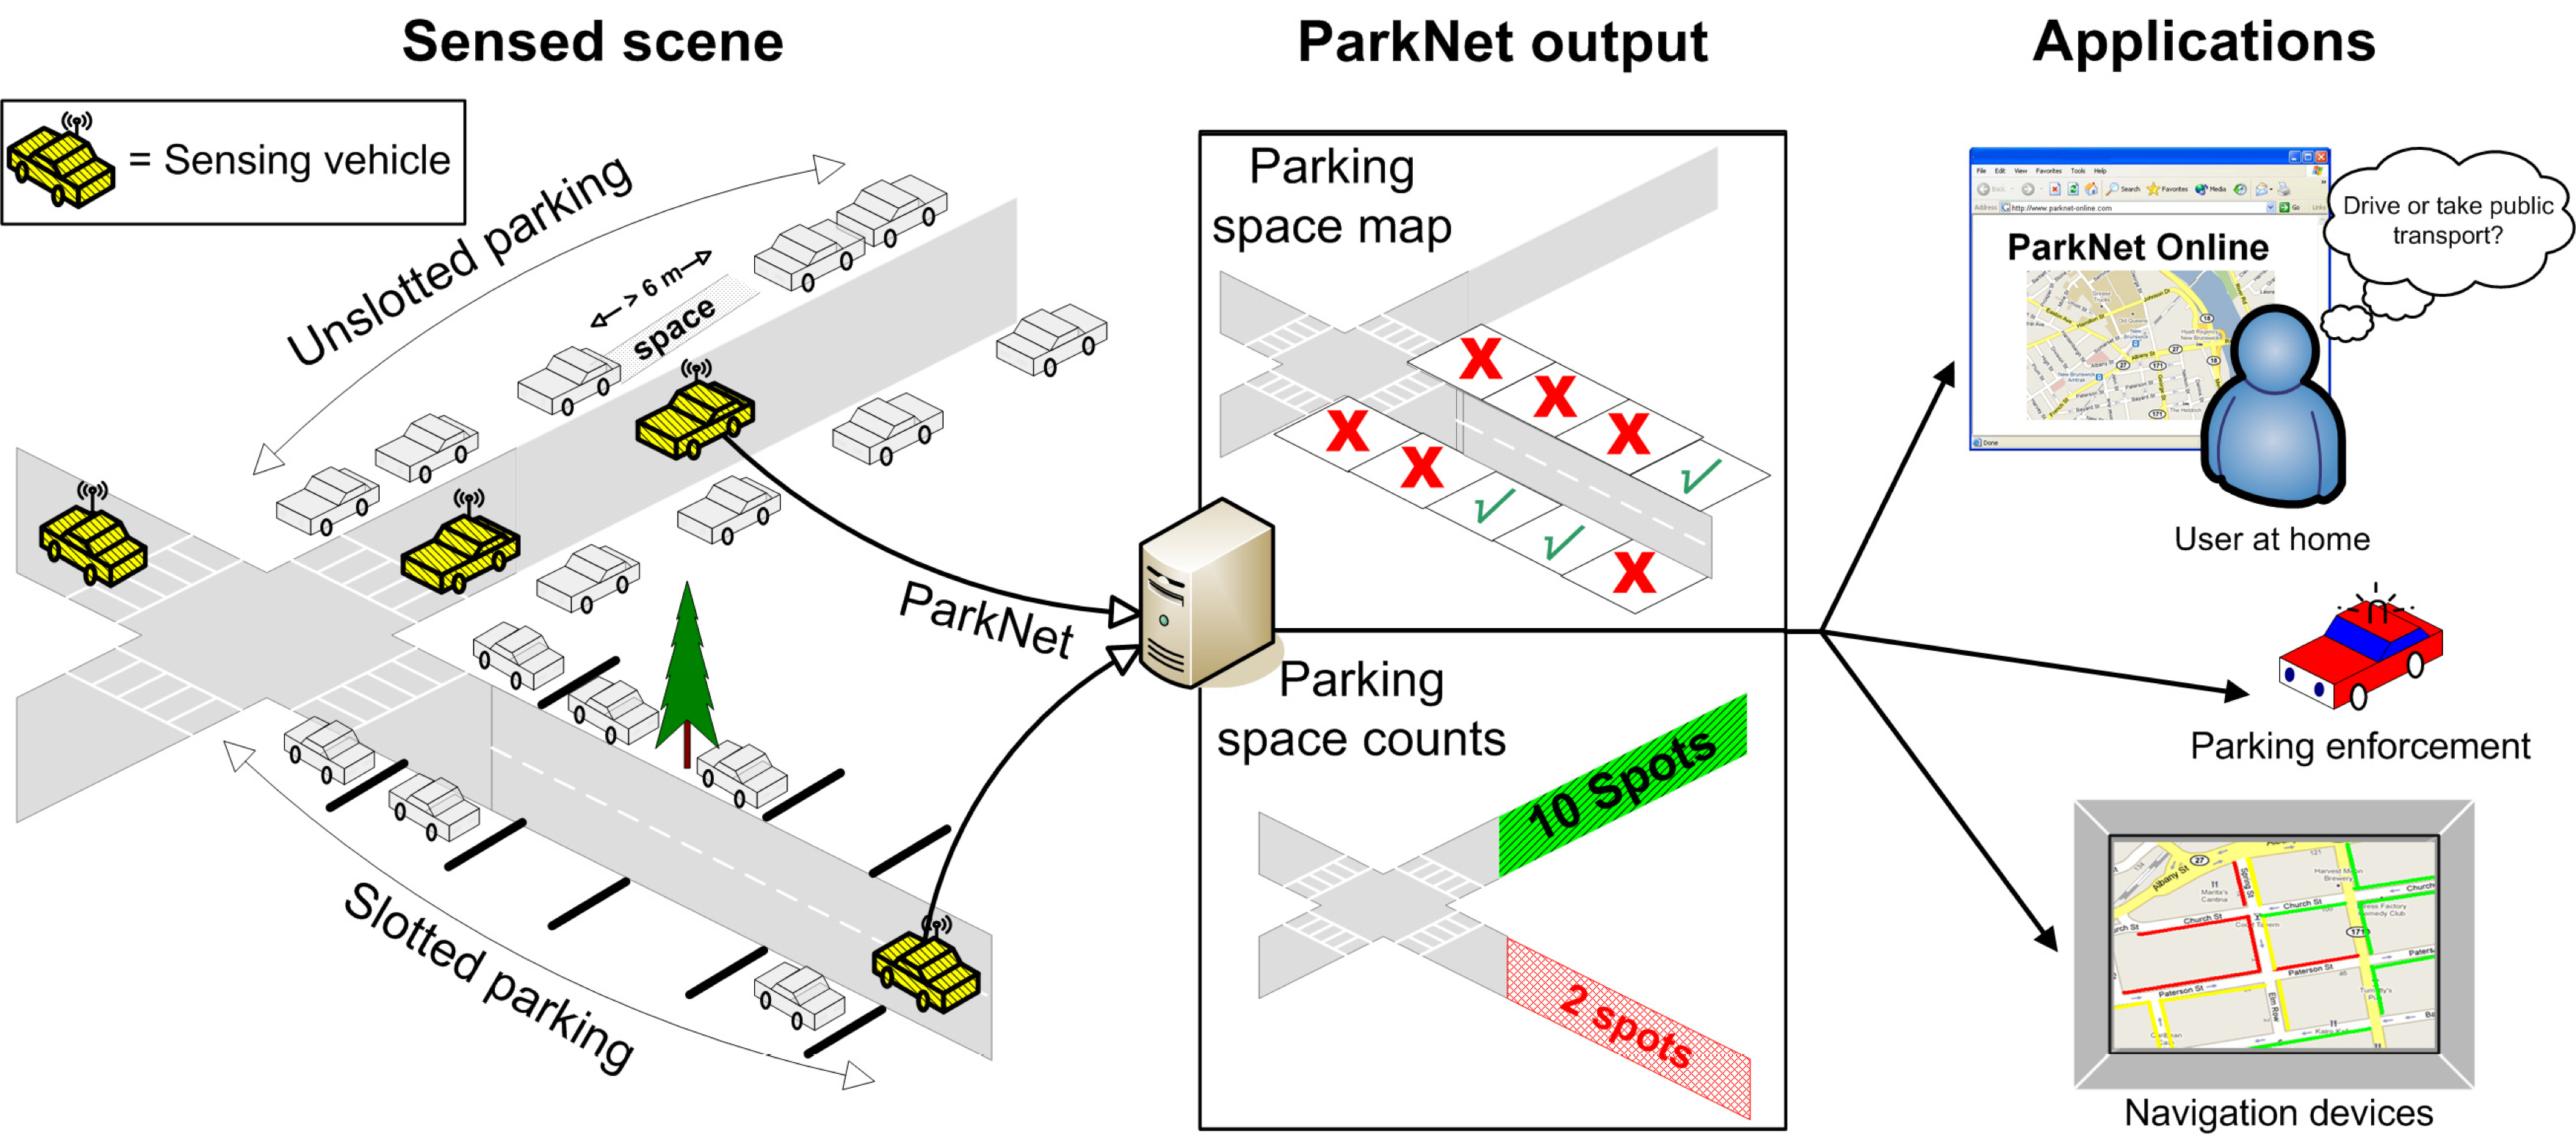
\includegraphics[width=13cm]{fig/parknet.png}
	\caption{MathurらによるParknet手法の概略図 \protect \footnotemark}
	\label{parknet-fig}
\end{figure}
\footnotetext{Parknetの資料\cite{Parknet}より引用}
MathurらによるParknetプロジェクトでは,車載センサーとGPSシステムを用いて路上駐車枠をセンシングする手法を提案している\cite{Parknet}.車両から得られたそれぞれの駐車枠の満空情報を,携帯電話回線網によって中央サーバーに収集する.それらのリアルタイムな情報から,中央サーバーが都市全体の路上駐車場のネットワークモデルを構築する.


また,CoricらはParknet手法に駐車禁止枠に対する違法駐車の検知機構を取り入れたアーキテクチャを提案している\cite{Crowdsensing}.この駐車禁止検知システムでは,90パーセント程度の推定精度が確認されている.

これらの手法の優位点は,路上に設置したセンサーに頼ること無くネットワークモデルの構築を動的に行える点にある.しかし,路上駐車場のみにフォーカスされており,敷地内駐車場に関してはまだ取り組むべき余地を残している.


\subsection{位置情報ログデータを用いた道路地図の推定手法}
\label{gps-gen-map}

スマートフォンやカーナビゲーションの移動ログデータの活用方法の一つとして,移動データから地図そのものを生成$\cdot$更新する取り組みが近年注目されている.ナビゲーションサービスの提供者にとって,地図を作成する費用を軽減出来る点だけではなく,急な通行止めや道路情報の変更にリアルタイムに柔軟な対応を可能にする点も大きなメリットになる.


\subsubsection{道路地図推定手法の分類と比較}
位置情報ログデータを用いる道路地図の推定に関して,様々な手法での提案が行われているが,Biagioniらによるサーベイ\cite{Biagioni}では大別して三つのアプローチに分類している.本節ではそれらの手法の分類と特徴について述べる.


\begin{itemize}
	\item k-Means法\\
	      \begin{figure}
	      	\centering
	      	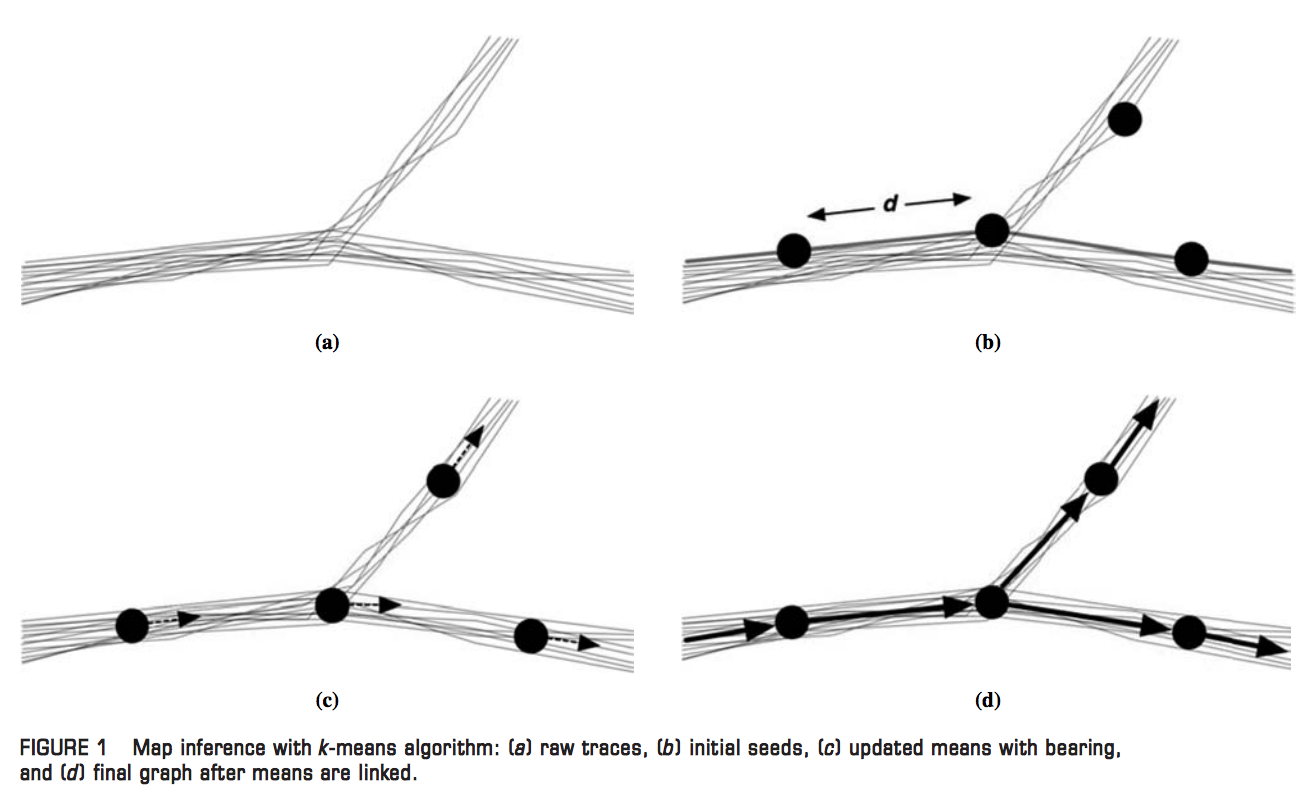
\includegraphics[width=10cm]{fig/kmeans-inf.png}
	      	\caption{k-Means法を用いる道路地図推定のフロー \protect \footnotemark}
	      	\label{k-means-inf}
          \end{figure}
          \footnotetext{Biagioniらの資料\cite{Biagioni}より引用}
	      k-Means法はForgeyらによって1965年に提唱されたクラスタリング手法である\cite{Forgy}.近年では多くの応用分野に取り入られている.道路地図の推定という文脈では,Edelkampらによって提案された手法\cite{Edelkamp}が著名である.
	      	      	      	      	      
	      図\ref{k-means-inf}に具体的なフローを示す.まず始めに,加工をしていない移動ログデータに初期シードを一定の間隔で設置し,k-Means法を用いてクラスタリングする.その後生成されたクラスターシードを,移動実績のある他のシードと結ぶことでエッジを生成する.これを繰り返すことで生成されたエッジから道路地図を推定することが出来る.
	      	      	      	      	      
	      	      	      	      	      
	\item Trace Merging法\\
	      \begin{figure}
	      	\centering
	      	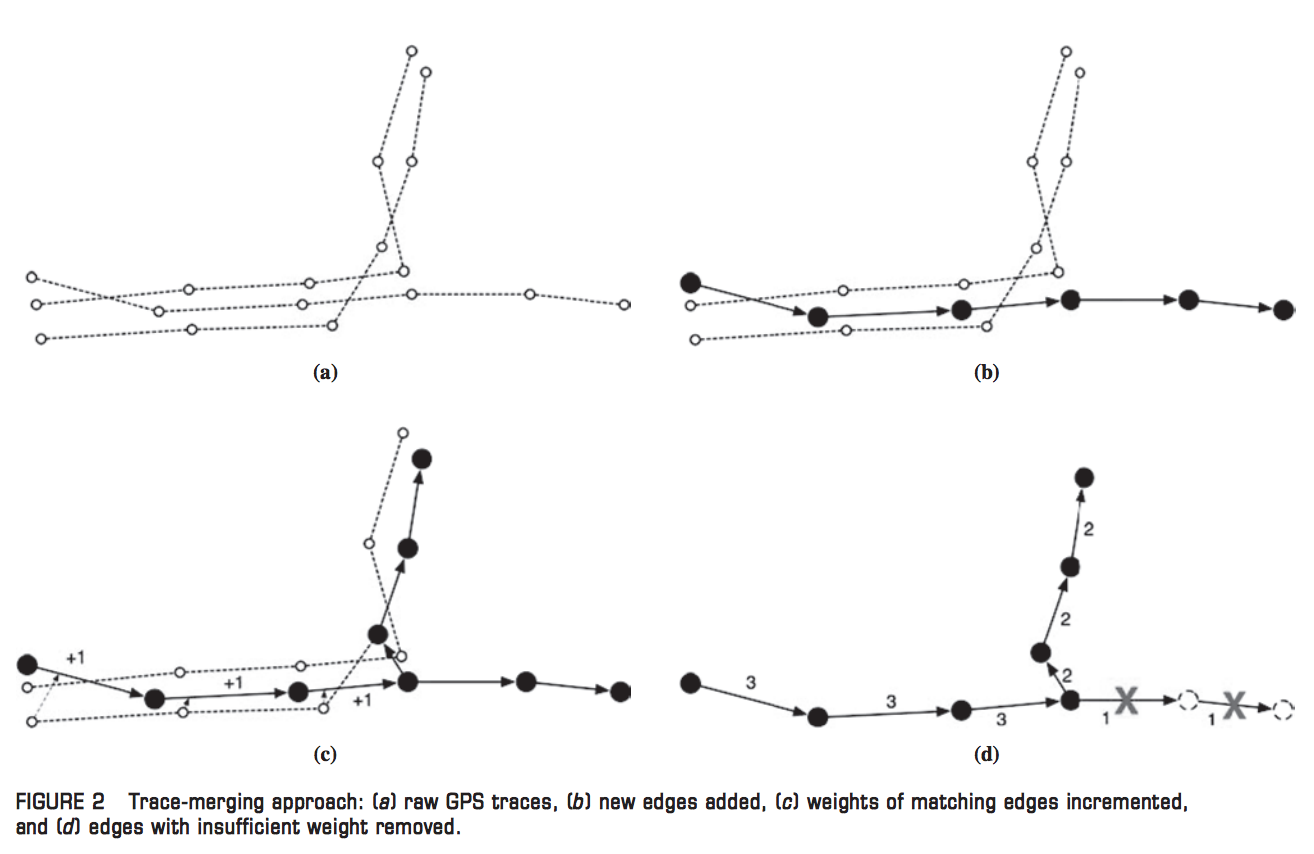
\includegraphics[width=10cm]{fig/trace-merging-inf.png}
	      	\caption{Trace Merging法を用いる道路地図推定のフロー \protect \footnotemark}
	      	\label{trace-merging-inf}
          \end{figure}
          \footnotetext{Biagioniらの資料\cite{Biagioni}より引用}
	      Caoらによって提案された手法がTrace Merging法である\cite{Cao}. 
	      この手法のフローを図\ref{trace-merging-inf}に示す.始めに,収集した位置情報ログデータをそれぞれ有向グラフとして表現する.次にこのグラフから一つを任意に選択し,このグラフのエッジの近傍で方向が一致するノード数をエッジの重みとして加算していく.最終的に残ったエッジから重みの少ない物を削除する.これにより,道路地図全体のネットワーク図が得られる.
	      	      	      	      	      
	\item カーネル密度推定法\\
	      \begin{figure}
	      	\centering
	      	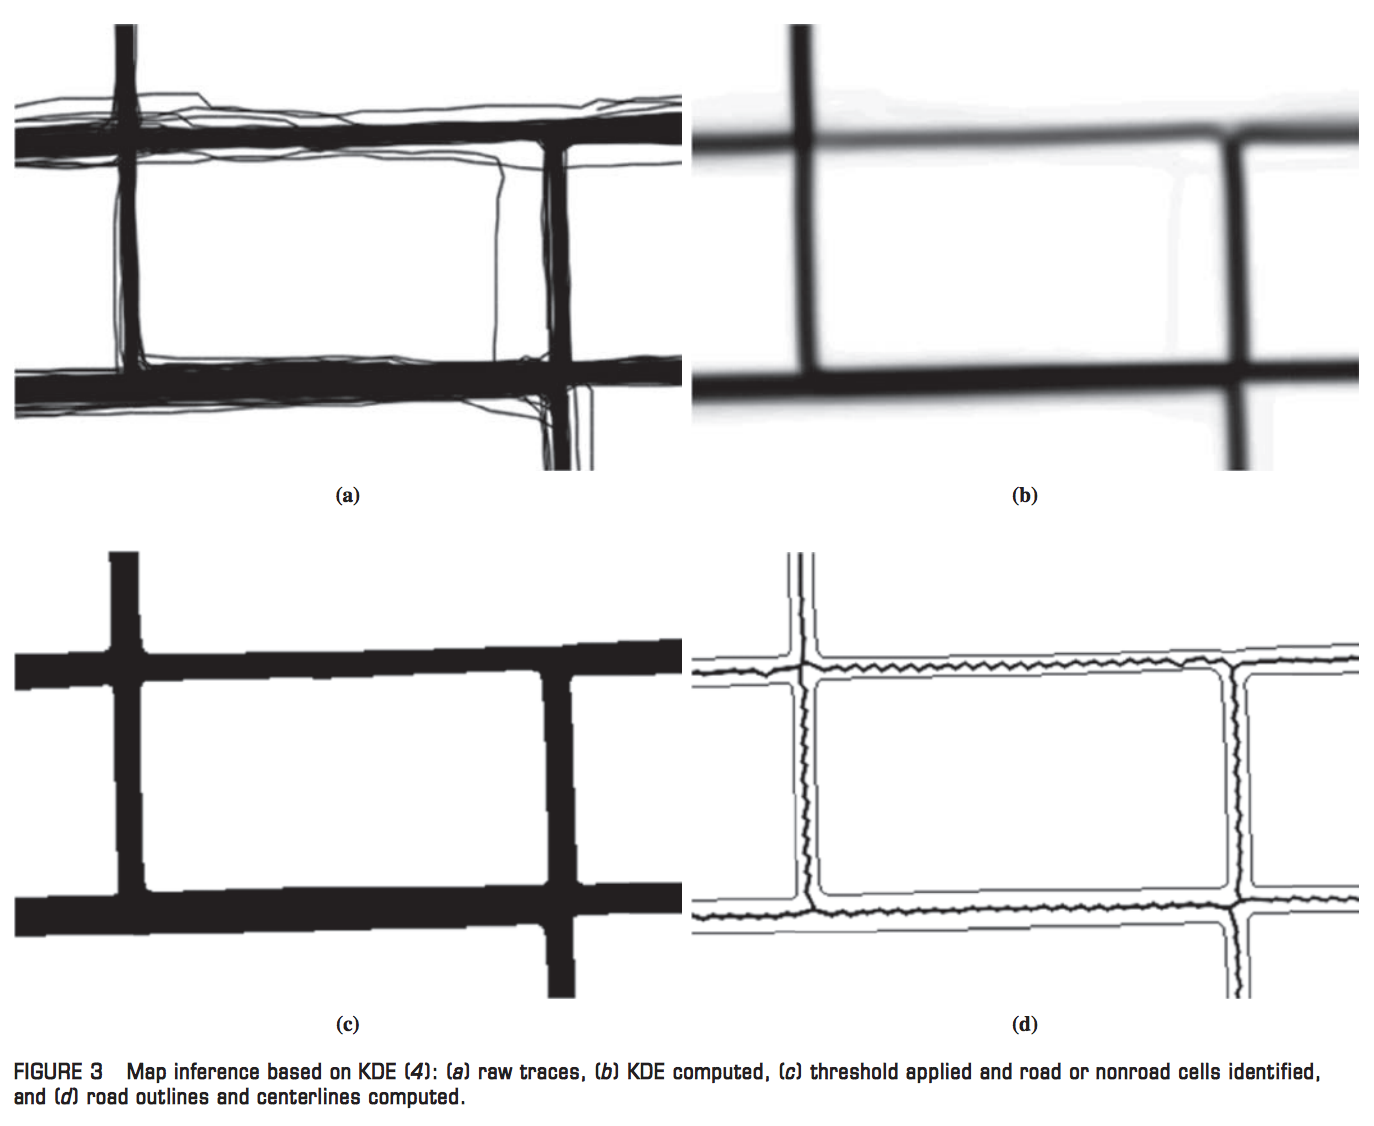
\includegraphics[width=10cm]{fig/kde-inf.png}
	      	\caption{カーネル密度推定を用いる道路地図推定のフロー \protect \footnotemark}
	      	\label{kde-inf}
          \end{figure}
          \footnotetext{Biagioniらの資料\cite{Biagioni}より引用}
	      Daviesらによってカーネル密度推定(以後KDE法)\cite{Ueki}を用いて道路地図推定を行う手法が提案されている\cite{Davies}.
	      	      	      	      	      
	      KDE法を用いるフローを図\ref{kde-inf}に示す.まず,元の移動ログ群からKDE法を用いて2Dヒストグラムを生成し,一定の閾値で二階長化する.生成された画像から道路の中心値群を結んで道路全体の地図を推定する.
	         	      	          
\end{itemize}

\begin{figure}[htb]
    \centering
    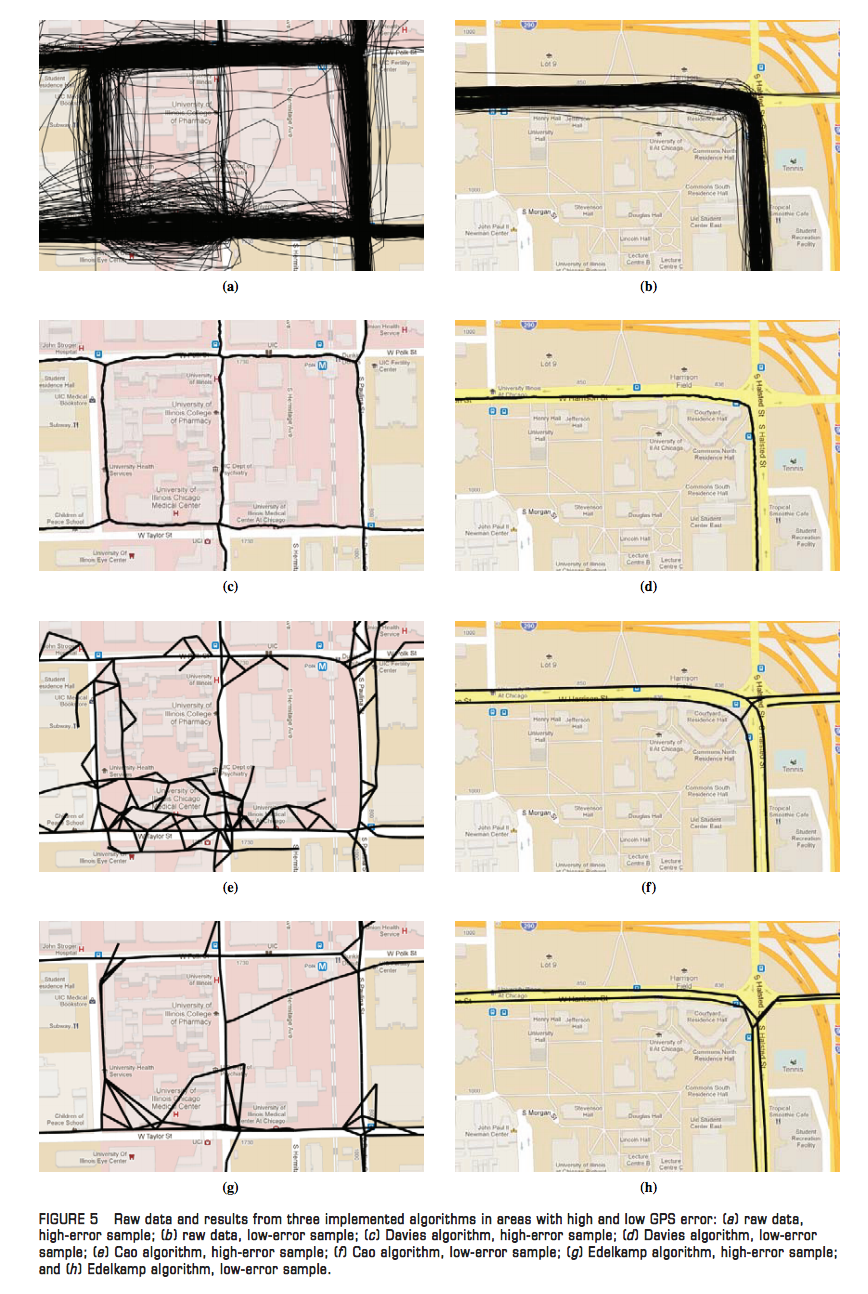
\includegraphics[width=10cm]{fig/inf-eval.png}
    \caption{k-Means法$\cdot$Trace Merging法$\cdot$KDE法の評価事例 \protect \footnotemark}
    \label{inf-eval}
\end{figure}
\footnotetext{{Biagioniらの資料\cite{Biagioni}より転載}}
こうした三つの手法を,実環境データにて評価した事例図\ref{inf-eval}に示す. 
                                            
ノイズの少ないログデータを用いた場合,三手法共に有効な結果を生成しているが,KDE法では移動量の少ない動線が捨象されやすいことが見て取れる.
                                        
一方,ノイズが多いログデータを用いた場合には,Trace Merging法とk-Means法では有意な類推が出来てない.他方,KDE法は捨象されている動線があるものの,真値に近い道路地図を推定していると判断可能である.
                                        
また,Biagioniらは各種法の実行時間に関しても言及している.100パターンの移動ログをデータセットとした場合,Trace Merging法が2.5時間の処理時間を要した一方で,k-Means法では73秒,KDE法では8秒と手法間で大きく差が開いている.加えて899パターンのデータセットを与えた場合において各手法の実行時間は,Trace Merging法では2.5日,k-Means法では15分,KDE法では25秒になった.締めくくりにBiagioniらはKDE法をベースとして各手法を組み合わせた新たな手法の提案について示唆している.

\subsubsection{三つの手法をあわせたアプローチについて}
Biaginiらは上記の三つの手法を組み合わせた新しいアプローチについての発表を行っている\cite{google-mouyatteta}.これによるとKDE法をベースとしたハイブリッドアプローチを用いることによって,より真値に近い道路地図の推定が可能になるとされている.


\section{車載アプリケーションプラットフォーム}
\label{ivi}
従来,自動車の情報端末はカーナビゲーションシステムとカーオーディオがその役割を担っていた.近年ではニーズの多様化やICT環境の発展によって,多くの情報からユーザーをサポートする役割も併せて求められるようになり,より高次元化されたIVI(車両情報端末) と総称される端末が登場している\cite{DICOMO}.多くのIVIプラットフォームでは,位置情報$\cdot$インターネットへのアクセス機構を備えており,自動車の情報を扱うための標準仕様の策定が活発である\cite{Ashimura}.例えば,WEB標準化団体であるW3CからはVehicle API\footnote{\url{https://www.w3.org/TR/vehicle-information-api/}}が提案されているほか,自動車メーカー各社からはスマートフォンとの連携機能を標準化するSmartDevicelink\footnote{\url{https://smartdevicelink.com/}}が提案されている.

